\documentclass[12pt,a4paper]{article}

\usepackage[utf8]{inputenc}
\usepackage[T1]{fontenc}
\usepackage[french]{babel}
\usepackage{amsmath,amssymb,amsthm}
\usepackage{cmbright}
\usepackage{exscale}
\usepackage[hidelinks]{hyperref}
\usepackage{cleveref}
\usepackage{graphicx}
\usepackage{tikz}
\usepackage{caption}
\usepackage{standalone}
\usetikzlibrary{decorations.pathreplacing}
\usepackage{tkz-tab}
\usepackage{xcolor}
\definecolor{accent}{HTML}{244470}
\usepackage{geometry}
\geometry{hmargin=2cm,vmargin=2cm}
\usepackage{enumitem}

\usepackage{titlesec}
\titleformat{\section}
{\color{accent}\Large\bfseries}
{\thesection.}
{0.8em}
{}
\titleformat{\subsection}
{\color{accent}\large\bfseries}
{\thesubsection}
{0.7em}
{}

\usepackage[many]{tcolorbox}
\tcbset{
navybar/.style={
enhanced,
colback=white,
colframe=accent,
boxrule=0.6pt,
leftrule=3pt,
arc=0pt,
outer arc=0pt,
left=8pt, right=8pt, top=6pt, bottom=6pt
},
graybar/.style={
enhanced,
colback=white,
colframe=gray!70,
boxrule=0.6pt,
leftrule=3pt,
arc=0pt,
outer arc=0pt,
left=8pt, right=8pt, top=6pt, bottom=6pt
},
}

\theoremstyle{plain}
\newtheorem{theorem}{Théorème}[section]
\newtheorem{property}[theorem]{Propriété}

\theoremstyle{definition}
\newtheorem{definition}[theorem]{Définition}
\newtheorem{example}[theorem]{Exemple}

\newtheorem{exercise}{Exercice}

\theoremstyle{remark}
\newtheorem*{remark}{Remarque}
\newtheorem*{recall}{Rappel}

\begin{document}

\noindent
\begin{minipage}[c]{0.62\textwidth}
  {\color{accent}\LARGE\bfseries Généralités sur les fonctions\par}
  \vspace{0.1cm}
  {\large 3\textsuperscript{ème} année secondaire\par}
  \vspace{0.7cm}
  {\bfseries \href{https://www.linkedin.com/in/kefrov/}{Fares Manai}\par}
  \vspace{2pt}
  {\small\href{mailto:kefrov630@gmail.com}{kefrov630@gmail.com}\par}
\end{minipage}
\hfill
\begin{minipage}[c]{0.33\textwidth}
  \centering
  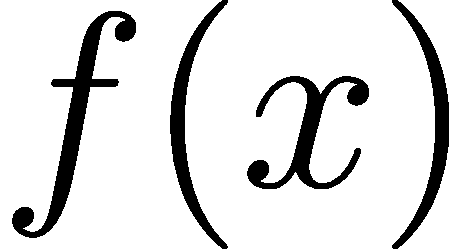
\includegraphics[width=\linewidth]{fx.pdf}
\end{minipage}
\par\vspace{0.4cm}
\noindent{\color{accent}\rule{\linewidth}{0.9pt}}
\par\vspace{0.5cm}

\tableofcontents

\newpage
\phantomsection
\section*{Introduction}
\addcontentsline{toc}{section}{Introduction}

\newpage
\section{Rappels}

\subsection{Fonctions}

\begin{tcolorbox}[navybar]
  \begin{definition}
    Soit $A$ et $B$ deux ensembles. Une fonction de $A$ vers $B$ est une règle
    qui associe à chaque élément $x \in A$ un seul élément de $B$.
    Cet élément de $B$ s'écrit $f(x)$. On dit que $f(x)$ est l'image de $x$
    par $f$, et que $x$ est un antécédent de $f(x)$. On écrit alors
    \[
    \begin{aligned}
      f : A &\rightarrow B \\
      x &\mapsto f(x).
    \end{aligned}
    \]
    L'ensemble $A$ s'appelle l'ensemble de définition de $f$, on le note aussi $D_f$,
    et $B$ s'appelle l'ensemble d'arrivée. L'ensemble image de $f$ est l'ensemble
    de toutes les valeurs que $f$ peut prendre :
    \[
    f(A) = \{y \in B \mid y = f(x) \text{ pour un certain } x \in A\}.
    \]
  \end{definition}
\end{tcolorbox}

La première chose à retenir : chaque entrée a une seule sortie.
Par exemple, dire que $f(x) = 1$ et $f(x) = 2$ pour le même $x$ n'a aucun sens,
d'après la définition d'une fonction. Par contre, une sortie peut venir de
plusieurs entrées : si $f(x) = x^2$, alors l'image de $3$ est $9$, et $9$ a deux
antécédents, $3$ et $-3$.

Deux fonctions qui ont la même expression mais des ensembles de définition
différents sont considérées comme différentes. Autrement dit, une fonction est
définie par son ensemble de définition et sa règle.

\begin{remark}
  Attention à ne pas confondre la fonction $f$ avec son expression $f(x)$.
  Notons aussi que l'ensemble image de $f$ n'est pas forcément égal à
  l'ensemble d'arrivée : c'est une partie de l'ensemble d'arrivée.
\end{remark}

Pour une fonction qui va d'une partie de $\mathbb{R}$ vers $\mathbb{R}$, on peut
faire un dessin, et cela est très utile pour l'étudier. D'où la définition suivante.
\begin{tcolorbox}[navybar]
  \begin{definition}
    Soit $(O, \vec{i}, \vec{j})$ un repère du plan. La courbe représentative d'une
    fonction $f : D_f \rightarrow \mathbb{R}$, notée $C_f$, est l'ensemble des points
    \[
    \{(x, f(x)) \mid x \in D_f\}.
    \]
  \end{definition}
\end{tcolorbox}

\begin{example}
  Il n'existe pas de fonction qui à chaque $x$ associe un $y$ avec la règle
  $y^2 = x$. En effet, pour $x > 0$, cette règle donne deux valeurs, $y$ et $-y$.
  Pour $x = 0$, elle en donne une seule, et pour $x < 0$, elle n'en donne aucune.
  Sur la Figure~\ref{fig:inverse_x_sq}, on a dessiné l'ensemble des points
  $(x,y)$ qui vérifient cette règle. Regardez la droite verticale d'équation
  $x=4$ : elle coupe la courbe en deux points, donc deux valeurs de $y$, $-2$ et $2$,
  correspondent à $x = 4$.

  Si on prend $y$ comme entrée et $x$ comme sortie, alors on peut définir une
  fonction, qui est simplement $y \mapsto y^2$.
\end{example}

\begin{example}
  Considérons les fonctions $f : \mathbb{R}_- \rightarrow \mathbb{R}$ et
  $g : \mathbb{R}_+ \rightarrow \mathbb{R}$ qui ont la même expression $x^2$.
  La Figure~\ref{fig:x_sq} montre que ces fonctions ne sont pas les mêmes, avec
  leurs courbes $C_f$ et $C_g$.
\end{example}

\begin{figure}[htbp]
  \centering
  \begin{minipage}[t]{0.43\linewidth}
    \centering
    \includestandalone[width=\linewidth]{figures/inverse_x_sq}
    \caption{$\{(x,y) \in \mathbb{R}^2 \mid y^2=x\}$.}
    \label{fig:inverse_x_sq}
  \end{minipage}\hfill
  \begin{minipage}[t]{0.42\linewidth}
    \centering
    \includestandalone[width=\linewidth]{figures/x_sq}
    \caption{$C_f$ et $C_g$.}
    \label{fig:x_sq}
  \end{minipage}
\end{figure}

\subsection{Valeur absolue}

Rappelons maintenant un opérateur très important, la valeur absolue, notée
$| \cdot |$. Elle est définie pour tout réel $x$ par :
\[
\lvert x \rvert =
\begin{cases}
  x & \text{si } x \ge 0 \\
  -x & \text{si } x < 0
\end{cases}
\]

En gros, pour tout $x$ non nul, elle renvoie la version positive de $x$.
Par exemple, $\lvert 3 \rvert = 3$ et $\lvert -3 \rvert = 3$. On peut aussi
la voir comme la \textit{distance} entre $x$ et $0$.

\begin{center}
  \includestandalone[width=0.6\linewidth]{figures/abs_example}
\end{center}

\begin{remark}
  Pour tout réel $x$, on a $\lvert x \rvert \ge 0$, et $\lvert x \rvert = 0$ si et
  seulement si $x = 0$. Cela se voit directement sur la définition, mais on va
  s'en servir plus tard.
\end{remark}

\begin{tcolorbox}[graybar]
\begin{property}
\label{prop:abs_opposite}
Pour tout $x \in \mathbb{R}$, on a $\lvert x \rvert = \lvert -x \rvert$.
\end{property}
\end{tcolorbox}

\begin{proof}
  On sépare trois cas. Si $x > 0$, alors $-x < 0$, donc
  $\lvert -x \rvert = -(-x) = x = \lvert x \rvert$.
  Si $x = 0$, alors $\lvert -x \rvert = \lvert 0 \rvert = 0 = \lvert x \rvert$.
  Si $x < 0$, alors $-x > 0$, donc $\lvert -x \rvert = -x = \lvert x \rvert$.
\end{proof}

On peut généraliser un peu l'idée de distance. Soit $a, b \in \mathbb{R}$.
Le nombre $\lvert a - b \rvert$ est la distance entre $a$ et $b$ sur la droite
des réels. Les nombres $\lvert a - b \rvert$ et $\lvert b - a \rvert$ représentent
la même distance. En effet, ils sont égaux d'après la
Propriété~\ref{prop:abs_opposite}, car $b - a = -(a - b)$.

\begin{center}
  \includestandalone[width=0.6\linewidth]{figures/abs_dis}
\end{center}

\begin{remark}
  Le plus souvent, pour enlever la valeur absolue, on découpe le problème en cas,
  selon le signe de la quantité qui est dans la valeur absolue.
\end{remark}

\begin{example}
  Écrivons $h(x) = \lvert x + 2 \rvert + \lvert x - 1 \rvert$ sans valeur absolue.
  On étudie d'abord le signe de chaque quantité qui est dans une valeur absolue :

  \begin{center}
  \begin{tikzpicture}
    \tkzTabInit[lgt=2, espcl=2.5, nocadre]
      {$x$ / 1, $x+2$ / 1, $x-1$ / 1}
      {$-\infty$, $-2$, $1$, $+\infty$}

    \tkzTabLine{, -, z, +, t, +}
    \tkzTabLine{, -, t, -, z, +}
  \end{tikzpicture}
  \end{center}

  On a donc trois cas.
  \begin{itemize}
    \item Si $x < -2$ : les deux quantités sont négatives, donc
    $\lvert x + 2 \rvert = -(x + 2)$ et $\lvert x - 1 \rvert = -(x - 1)$.
    On obtient $h(x) = -2x - 1$.
    \item Si $-2 \le x \le 1$ : on a $x + 2 \ge 0$ et $x - 1 \le 0$, donc
    $h(x) = (x + 2) - (x - 1) = 3$.
    \item Si $x > 1$ : les deux quantités sont positives, donc
    $h(x) = (x + 2) + (x - 1) = 2x + 1$.
  \end{itemize}
  Autrement dit,
  \[
    h(x) =
    \begin{cases}
      -2x - 1 & \text{si } x < -2 \\
      3 & \text{si } -2 \le x \le 1 \\
      2x + 1 & \text{si } x > 1.
    \end{cases}
  \]
  Vérifions avec $x = 3$ : d'un côté $\lvert 5 \rvert + \lvert 2 \rvert = 7$,
  de l'autre $2 \cdot 3 + 1 = 7$.
\end{example}

\begin{tcolorbox}[graybar]
\begin{property}
  \label{prop:abs_ab}
  Pour tous $a, b \in \mathbb{R}$, on a $\lvert ab \rvert = \lvert a \rvert
  \lvert b \rvert$.
\end{property}
\end{tcolorbox}

\begin{proof}
  Cette preuve est laissée au lecteur.
\end{proof}

On se demande maintenant quelles valeurs de $x$ vérifient $\lvert x \rvert \le r$
pour un certain $r \ge 0$. On utilise encore la droite des réels pour guider
notre intuition : on place les points $r$ et $-r$, on choisit plusieurs valeurs
de $x$, on regarde où tombe leur valeur absolue, puis on généralise.

\begin{center}
  \includestandalone[width=0.78\linewidth]{figures/abs_ineq}
\end{center}

\begin{tcolorbox}[graybar]
  \begin{property}
    Soit $r \ge 0$. L'ensemble des réels $x$ qui vérifient $\lvert x \rvert \le r$
    est l'intervalle $[-r, r]$. Autrement dit,
    \[
      \lvert x \rvert \le r \Longleftrightarrow -r \le x \le r.
    \]
  \end{property}
\end{tcolorbox}

\begin{proof}
  On sépare deux cas.

  Si $x \ge 0$, alors $\lvert x \rvert = x$, donc $\lvert x \rvert \le r$ revient à
  $x \le r$. Or $-r \le 0 \le x$ est toujours vrai, donc $x \le r$ revient à
  $-r \le x \le r$.

  Si $x < 0$, alors $\lvert x \rvert = -x$, donc $\lvert x \rvert \le r$ revient à
  $-x \le r$, c'est-à-dire $x \ge -r$. Or $x < 0 \le r$ est toujours vrai, donc
  $x \ge -r$ revient à $-r \le x \le r$.

  Ces deux cas couvrent tous les réels, donc l'équivalence est vraie pour tout $x$.
\end{proof}

\begin{remark}
  Cette propriété reste vraie quand on remplace $x$ par une expression. Par exemple,
  $\lvert x - 3 \rvert \le 2 \Longleftrightarrow -2 \le x - 3 \le 2
  \Longleftrightarrow 1 \le x \le 5$. En particulier, pour $a \in \mathbb{R}$ et
  $r \ge 0$,
  \[
    \lvert x - a \rvert \le r \Longleftrightarrow a - r \le x \le a + r.
  \]
  C'est logique : ce sont exactement les réels $x$ dont la distance à $a$ est
  au plus $r$.
\end{remark}

On termine cette sous-section avec la courbe de la fonction valeur absolue
$x \mapsto \lvert x \rvert$. Utilisez la Figure~\ref{fig:abs_func} pour la comparer
avec la fonction identité $x \mapsto x$.

\begin{figure}[ht]
  \centering
  \includestandalone[width=0.43\linewidth]{figures/abs_func}
  \caption{Les courbes de $x \mapsto x$ et $x \mapsto \lvert x \rvert$.}
  \label{fig:abs_func}
\end{figure}

\subsection{Racine carrée}

\begin{tcolorbox}[navybar]
\begin{definition}
  Soit $a \ge 0$. Une racine carrée de $a$ est un nombre positif, noté
  $\sqrt{a}$, tel que
  \[
    (\sqrt{a})^2 = a.
  \]
\end{definition}
\end{tcolorbox}

On admet qu'un tel nombre existe toujours. On insiste sur $a \ge 0$ : l'opérateur
racine carrée, noté $\sqrt{\cdot}$, ne s'applique qu'aux réels de $\mathbb{R}_+$,
car le carré d'un réel est toujours positif.

Prouvons l'unicité de la racine carrée. Prenons deux nombres $x, y \ge 0$ tels que
$x^2 = a$ et $y^2 = a$. On obtient
\[
  \begin{aligned}
    x^2 &= y^2 \\
    x^2 - y^2 &= 0 \\
    (x - y)(x + y) &= 0,
  \end{aligned}
\]
ce qui donne $x = y$ ou $x = -y$ (un produit est nul si l'un des facteurs est nul).
Dans le premier cas, c'est fini : on a bien $x = y$. Dans le second cas, comme
$x \ge 0$ et $-y \le 0$, l'égalité $x = -y$ n'est possible que si $x = y = 0$.
On a donc encore $x = y$. Il n'y a ainsi qu'un seul nombre positif dont le carré
vaut $a$ : on peut parler de \textit{la} racine carrée de $a$. On utilise ce fait
pour prouver la propriété suivante.

\begin{tcolorbox}[graybar]
\begin{property}
  Pour tous $a, b \ge 0$, on a $\sqrt{ab} = \sqrt{a}\sqrt{b}$.
\end{property}
\end{tcolorbox}

\begin{proof}
  Le nombre $\sqrt{a}\sqrt{b}$ est positif, et on a
  $(\sqrt{a}\sqrt{b})^2 = (\sqrt{a})^2(\sqrt{b})^2 = ab$.
  Par unicité de $\sqrt{ab}$, on conclut que $\sqrt{ab} = \sqrt{a}\sqrt{b}$.
\end{proof}

\begin{remark}
  En général, $\sqrt{a + b} \neq \sqrt{a} + \sqrt{b}$. À vous de jouer : vérifiez
  que l'égalité est fausse pour $a = 9$ et $b = 16$.
\end{remark}

À première vue, on est tenté d'écrire $\sqrt{a^2} = a$ pour un réel $a$, mais
regardez le cas $a < 0$. Par exemple, pour $a = -3$, on a $a^2 = 9$ et
$\sqrt{9} = 3$, pas $-3$. Il est vrai que $a \cdot a = a^2$, mais la racine carrée
doit être positive. Donc $\sqrt{a^2}$ n'est pas toujours égal à $a$.
Ne faites pas cette erreur très classique.

\begin{tcolorbox}[graybar]
\begin{property}
  Pour tout réel $a$, on a $\sqrt{a^2} = \lvert a \rvert$.
\end{property}
\end{tcolorbox}

\begin{proof}
  D'après la Propriété~\ref{prop:abs_ab}, on peut écrire
  $\lvert a \rvert \lvert a \rvert = \lvert a \cdot a \rvert = \lvert a^2 \rvert$.
  Comme $a^2 \ge 0$, on a $\lvert a^2 \rvert = a^2$. On obtient donc
  $\lvert a \rvert^2 = a^2$. De plus, $\lvert a \rvert \ge 0$, comme on l'a
  remarqué plus haut. Par unicité de la racine carrée, $\sqrt{a^2} = \lvert a \rvert$.
\end{proof}

Comme dans la sous-section précédente, on termine avec la
Figure~\ref{fig:sq_func}, qui montre la fonction racine carrée définie sur
$\mathbb{R}_+$. Son graphe est en fait la moitié supérieure ($y \ge 0$) du graphe
de la Figure~\ref{fig:inverse_x_sq}.

\begin{figure}[ht]
  \centering
  \includestandalone[width=0.53\linewidth]{figures/sq_func}
  \caption{Courbe de $x \mapsto \sqrt{x}$.}
  \label{fig:sq_func}
\end{figure}

\subsection{Polynômes}

Le polynôme est l'une des premières fonctions particulières que l'on rencontre.
Les polynômes sont très importants et très utiles grâce à leur simplicité.

\begin{tcolorbox}[navybar]
  \begin{definition}
    Une fonction $p : \mathbb{R} \rightarrow \mathbb{R}$ est un polynôme
    si, pour tout $x \in \mathbb{R}$, son expression est de la forme
    \[
    p(x) = a_0 + a_1 x + a_2 x^2 + \cdots + a_m x^m,
    \]
    où $a_0, \dots, a_m \in \mathbb{R}$.
  \end{definition}
\end{tcolorbox}

En 2\textsuperscript{ème} année secondaire, on a surtout étudié les polynômes où
$m = 2$. On dit que ces polynômes sont du second degré.

\begin{tcolorbox}[navybar]
  \begin{definition}
    Un polynôme $p$ est de degré $m$ si, pour tout $x \in \mathbb{R}$,
    son expression est de la forme
    \[
    p(x) = a_0 + a_1 x + a_2 x^2 + \cdots + a_m x^m,
    \]
    où $a_0, \dots, a_m \in \mathbb{R}$ et $a_m \neq 0$.

    Par convention, le degré du polynôme nul n'est pas défini.
  \end{definition}
\end{tcolorbox}

On s'est aussi beaucoup intéressé aux racines des polynômes de degré $2$.

\begin{tcolorbox}[navybar]
  \begin{definition}
    Les racines d'un polynôme $p$ sont les réels $x$ tels que $p(x) = 0$.
  \end{definition}
\end{tcolorbox}

\noindent
\begin{minipage}[c]{0.5\linewidth}
  \begin{example}
    Considérons l'équation du second degré
    \[
      p(x) = x^2 - 5x + 6 = 0.
    \]
    Graphiquement, comme le montre la Figure~\ref{fig:poly_roots},
    les racines sont $2$ et $3$. On peut aussi le vérifier facilement :
    $p(2) = 4 - 10 + 6 = 0$ et $p(3) = 9 - 15 + 6 = 0$.

    Une question se pose pourtant : comment trouver les racines de façon
    \textit{sûre}, i.e., sans utiliser la courbe de $p$ ?
    \label{eg:poly_roots}
  \end{example}
\end{minipage}\hfill
\begin{minipage}[c]{0.42\linewidth}
  \captionsetup{hypcap=false, skip=12pt}

  \begin{minipage}[c][6cm][c]{\linewidth}
    \centering
    \includestandalone[width=\linewidth]{figures/poly_roots}
  \end{minipage}

  \captionof{figure}{Racines de $x^2 - 5x + 6$.}
  \label{fig:poly_roots}
\end{minipage}
\par
\vspace{0.5em}

Considérons l'équation $ax^2 + bx + c = 0$ avec $a \neq 0$. Graphiquement, en
imaginant certaines translations de la parabole, on peut prévoir qu'une telle
équation a soit 0, soit 1, soit 2 solutions. Ces solutions sont les racines du
polynôme $ax^2 + bx + c$. Une question naturelle se pose : dans quels cas
a-t-on chacune de ces situations, et quelle est la forme des racines ?

On remarque qu'il y a deux termes qui contiennent $x$ : $ax^2$ et $bx$.
L'idée est de réécrire l'expression pour qu'il n'y ait qu'un seul $x$ au lieu de
deux. Observons l'identité remarquable
\[
(x + A)^2 = x^2 + A^2 + 2Ax.
\]
À gauche, il y a un seul $x$, alors qu'à droite il y en a deux. En essayant
d'en profiter pour notre équation, on obtient
\[
\begin{aligned}
  x^2 + \frac{b}{a}x + \frac{c}{a} &= 0 \quad \text{(on divise par } a \neq 0 \text{)} \\
  x^2 + 2\left(\frac{b}{2a}\right)x + \frac{c}{a} &= 0 \quad \text{(on réécrit le terme du milieu)} \\
  x^2 + 2\left(\frac{b}{2a}\right)x + \left(\frac{b}{2a}\right)^2 - \left(\frac{b}{2a}\right)^2 + \frac{c}{a} &= 0 \quad \text{(on ajoute et on retire le même carré)} \\
  \left(x + \frac{b}{2a}\right)^2 - \frac{b^2}{4a^2} + \frac{c}{a} &= 0 \quad \text{(on factorise le carré parfait)} \\
  \left(x + \frac{b}{2a}\right)^2 - \frac{b^2 - 4ac}{4a^2} &= 0 \quad \text{(on met au même dénominateur)} \\
  \left(x + \frac{b}{2a}\right)^2 &= \frac{b^2 - 4ac}{4a^2}
\end{aligned}
\]

On a exactement ce que l'on voulait : un seul $x$ du côté gauche. Le nombre
$b^2 - 4ac$ est tellement important qu'il a un nom : le discriminant, noté $\Delta$.
\[
\left(x + \frac{b}{2a}\right)^2 = \frac{\Delta}{4a^2}
\]

Le côté gauche est un carré, donc il est positif. Comme $4a^2$ est strictement
positif, le nombre de solutions réelles dépend uniquement du signe de $\Delta$.
On obtient donc 3 cas :

\begin{itemize}
  \item Si $\Delta < 0$ : le côté droit est négatif. Un carré ne peut pas être
  négatif, donc il y a 0 solution.
  \item Si $\Delta = 0$ : le côté droit est nul. Donc $x + \frac{b}{2a} = 0$, ce qui
  donne exactement 1 solution (une racine double) :
  \[
  x = -\frac{b}{2a}
  \]
  \item Si $\Delta > 0$ : on peut prendre la racine carrée des deux côtés. Comme
  $\frac{\Delta}{4a^2} = \Delta \left(\frac{1}{2a}\right)^2$, les propriétés de
  la racine carrée donnent
  \[
    \sqrt{\frac{\Delta}{4a^2}} = \sqrt{\Delta}\,\sqrt{\left(\frac{1}{2a}\right)^2}
    = \sqrt{\Delta}\,\left\lvert\frac{1}{2a}\right\rvert = \frac{\sqrt{\Delta}}{2\lvert a \rvert}.
  \]
  Le signe $\pm$ nous permet de remplacer $\lvert a \rvert$ par $a$ : si $a < 0$,
  les deux nombres $\pm\frac{\sqrt{\Delta}}{2\lvert a \rvert}$ sont les mêmes
  que $\pm\frac{\sqrt{\Delta}}{2a}$, juste dans l'autre ordre. On obtient 2 solutions,
  notées $x_1$ et $x_2$, et la célèbre formule :
  \[
  \begin{aligned}
    x + \frac{b}{2a} &= \pm \frac{\sqrt{\Delta}}{2a} \\
    x &= \frac{-b \pm \sqrt{\Delta}}{2a}.
  \end{aligned}
  \]
\end{itemize}

Vous pouvez maintenant revenir vérifier cette formule dans l'Exemple~\ref{eg:poly_roots}.
On remarque aussi sur la Figure~\ref{fig:poly_roots} que pour les valeurs de $x$
entre $x_1$ et $x_2$, les valeurs de $p(x)$ sont toutes négatives. Cette
observation nous pousse à chercher le lien entre les racines d'un polynôme du
second degré et son signe. Pour cela, on aura besoin du théorème suivant.

\begin{tcolorbox}[navybar]
\begin{theorem}
  Soit $p$ un polynôme de degré $m \in \mathbb{N}^*$ et $\lambda \in \mathbb{R}$.
  Alors $p(\lambda) = 0$ si et seulement s'il existe un polynôme $q$ de degré
  $m - 1$ tel que
  \[
    p(x) = (x - \lambda)q(x)
  \]
  pour tout $x \in \mathbb{R}$.
\end{theorem}
\end{tcolorbox}

\begin{proof}
  Exercice~??.
\end{proof}

\begin{example}
  Considérons le polynôme du second degré $p(x) = x^2 - 5x + 6$. On sait déjà,
  grâce à la Figure~\ref{fig:poly_roots}, que ses racines sont $x_1 = 2$ et $x_2 = 3$.

  D'après le théorème précédent, comme $p(2) = 0$, il existe un polynôme $q$
  de degré $1$ tel que
  \[
    p(x) = (x - 2)q(x).
  \]

  Appliquons le théorème une deuxième fois pour trouver $q$. On calcule $p$ en
  l'autre racine, $x = 3$ :
  \[
    p(3) = (3 - 2)q(3) \implies 0 = 1 \cdot q(3) \implies q(3) = 0.
  \]
  Comme $q(3) = 0$, le théorème dit qu'il existe un polynôme $r$ de degré
  $1 - 1 = 0$ tel que $q(x) = (x - 3)r(x)$.

  Un polynôme de degré $0$ est simplement une constante, donc $r(x) = a$ pour un
  certain réel $a$. En remplaçant, on obtient
  \[
    p(x) = a(x - 2)(x - 3).
  \]
  Si on développe le côté droit, le terme de plus haut degré est $ax^2$. Or
  $p(x) = x^2 - 5x + 6$ a pour coefficient de $x^2$ le nombre $1$. Par
  identification (on admet que deux polynômes égaux ont les mêmes coefficients),
  on a $a = 1$. On obtient donc la factorisation complète :
  \[
    p(x) = (x - 2)(x - 3).
  \]

  Le signe de $p(x)$ dépend des signes de ses deux facteurs. En étudiant le signe
  de chaque facteur séparément, on peut construire le tableau de signes suivant :

  \begin{center}
  \begin{tikzpicture}
    \tkzTabInit[lgt=2, espcl=2.5, nocadre]
      {$x$ / 1, $x-2$ / 1, $x-3$ / 1, $p(x)$ / 1}
      {$-\infty$, $2$, $3$, $+\infty$}

    \tkzTabLine{, -, z, +, t, +}
    \tkzTabLine{, -, t, -, z, +}
    \tkzTabLine{, +, z, -, z, +}
  \end{tikzpicture}
  \end{center}

  Comme on s'y attendait avec le graphe de $p$, on a $p(x) > 0$ pour
  $x \in ]-\infty, 2[ \,\cup\, ]3, +\infty[$, on a $p(x) < 0$ pour
  $x \in ]2, 3[$, et $p(x) = 0$ pour $x = 2$ et $x = 3$.
\end{example}

\begin{example}
  Considérons maintenant $p(x) = x^2 - 4x + 4$. Ici,
  $\Delta = (-4)^2 - 4 \times 1 \times 4 = 0$, donc il y a une seule racine,
  $x = 2$. On reconnaît aussi une identité remarquable :
  \[
    p(x) = (x - 2)^2.
  \]
  Le facteur $x - 2$ apparaît deux fois, c'est pour cela qu'on parle de racine
  double. Voici le tableau de signes :

  \begin{center}
  \begin{tikzpicture}
    \tkzTabInit[lgt=2, espcl=2.5, nocadre]
      {$x$ / 1, $x-2$ / 1, $p(x)$ / 1}
      {$-\infty$, $2$, $+\infty$}

    \tkzTabLine{, -, z, +}
    \tkzTabLine{, +, z, +}
  \end{tikzpicture}
  \end{center}

  Le polynôme $p$ est donc toujours positif, et il s'annule seulement en $2$.
  À part en sa racine double, il a le signe de son coefficient de $x^2$, qui
  est $1$.
\end{example}

\begin{example}
  Considérons enfin $p(x) = -x^2 + 2x - 2$. Ici,
  $\Delta = 2^2 - 4 \times (-1) \times (-2) = 4 - 8 = -4 < 0$, donc $p$ n'a
  aucune racine, et on ne peut pas le factoriser comme avant. Pour trouver son
  signe, on refait l'idée de tout à l'heure : faire apparaître un carré.
  \[
    p(x) = -(x^2 - 2x + 2) = -\left((x - 1)^2 + 1\right).
  \]
  Comme $(x - 1)^2 \ge 0$, on a $(x - 1)^2 + 1 \ge 1 > 0$. Donc $p(x) < 0$ pour
  tout réel $x$ : le polynôme garde toujours le signe de son coefficient de
  $x^2$, qui est $-1$. Voici le tableau de signes :

  \begin{center}
  \begin{tikzpicture}
    \tkzTabInit[lgt=2, espcl=4, nocadre]
      {$x$ / 1, $p(x)$ / 1}
      {$-\infty$, $+\infty$}

    \tkzTabLine{, -}
  \end{tikzpicture}
  \end{center}
\end{example}

\subsection{Fonctions rationnelles}

\begin{tcolorbox}[navybar]
  \begin{definition}
    Une fonction rationnelle est une fonction $f$ qui peut s'écrire comme le
    quotient de deux polynômes :
    \[
      f(x) = \frac{p(x)}{q(x)}
    \]
    où $p$ et $q$ sont des polynômes, et $q$ n'est pas le polynôme nul.
  \end{definition}
\end{tcolorbox}

Comme diviser par zéro n'a pas de sens, une fonction rationnelle $x \mapsto f(x)$
n'est définie que pour les $x$ où le polynôme $q$ ne s'annule pas. Autrement dit,
\[
  D_f = \{x \in \mathbb{R} \mid q(x) \neq 0\}.
\]

\begin{remark}
  Les polynômes sont des fonctions rationnelles particulières : il suffit de
  prendre pour $q$ le polynôme constant égal à $1$.
\end{remark}

\begin{example}
  Considérons $x \mapsto 1/x$. C'est la première fonction rationnelle que l'on
  étudie, et sans doute la plus importante et la plus utile. Son ensemble de
  définition est $\mathbb{R}^*$, car $x \neq 0$. Voir la
  Figure~\ref{fig:rational_func1} pour son graphe.
\end{example}

\begin{example}
  Considérons la fonction suivante, définie sur $\mathbb{R} \setminus \{1\}$ :
  \[
    f(x) = \frac{x^2 - 1}{x - 1}.
  \]
  Remarquons que, pour tout $x \neq 1$, on a
  $\frac{x^2 - 1}{x - 1} = \frac{(x - 1)(x + 1)}{x - 1} = x + 1$.
  Il ne faut pas aller trop vite et confondre $f$ avec $x \mapsto x + 1$ : ce
  sont deux fonctions différentes, car elles n'ont pas le même ensemble de
  définition. Par exemple, $f(1)$ n'existe pas, alors que l'image de $1$ par
  $x \mapsto x + 1$ est $2$.
\end{example}

\begin{example}
  Considérons la fonction $g(x) = \frac{x^2 + 1}{x}$. Son ensemble de définition
  est $D_g = \mathbb{R} \setminus \{0\}$. On peut réécrire l'expression :
  \[
    g(x) = x + \frac{1}{x}.
  \]
  Quand $x$ devient très grand en valeur absolue, $\frac{1}{x}$ se rapproche de $0$.
  Par exemple, pour $x = 1000$, on a $\frac{1}{x} = 0.001$ et $g(x) = 1000.001$.
  Donc le graphe de $g$ se rapproche de plus en plus de la droite oblique $y = x$,
  comme on le voit sur la Figure~\ref{fig:rational_func2}.
\end{example}

\begin{figure}[htbp]
  \centering
  \begin{minipage}[t]{0.42\linewidth}
    \centering
    \includestandalone[width=\linewidth]{figures/rational_func1}
    \caption{Courbe de $x \mapsto 1/x$.}
    \label{fig:rational_func1}
  \end{minipage}\hfill
  \begin{minipage}[t]{0.42\linewidth}
    \centering
    \includestandalone[width=\linewidth]{figures/rational_func2}
    \caption{Courbe de $x \mapsto x + \frac{1}{x}$.}
    \label{fig:rational_func2}
  \end{minipage}
\end{figure}

\newpage
\section{Translations de graphes}



\newpage
\phantomsection
\section*{Conclusion}
\addcontentsline{toc}{section}{Conclusion}

\end{document}
